\chapter{System design}

\href{https://github.com/AnotherGitAccount/TFE/blob/master/hardware/DE10_NANO_SoC_GHRD.v}{Github link to the GHRD file.}

In this chapter the final steps of the system design are described. The generation of the HPS 
system allowing the connection between the FPGA and the ARM processor, the interconnection of the 
different super units as well as the installation of the system on the FPGA and the OS on the 
ARM processor are detailed.

\section{Generating the HPS module}

In the previous sections, the ARM-FPGA interconnect was described using QSys. Now that all the 
required elements have been defined, all that remains is to generate the HPS system from QSys. 
This is done simply by pressing the generate button and choosing Verilog as output language in QSys.
This operation generates a module that can be used in the project. In fact, the module gives access 
to all the signals exported to QSys (as input or output depending on the signal). In addition to 
that, some signals such as reset, clock, etc. are present in the module interface. Inside the HPS 
module are the different modules that have been added in QSys (PIO and Avalon to external bus bridge) 
as well as other modules necessary for the operation of the interconnection. The HPS is also 
connected to the different FPGA-ARM bridges inside. The interface of the HPS is given in 
Figure \ref{fig:system/hps}.

\begin{figure}[H]
    \centering
    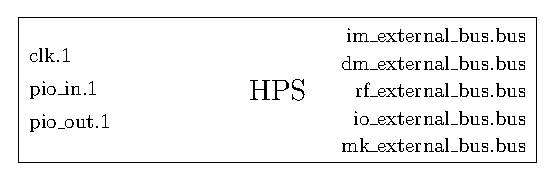
\includegraphics[scale=0.8]{Chapter6-System/res/hps.eps}
    \caption{HPS system.}
    \label{fig:system/hps}
\end{figure}

\section{Golden Hardware Reference Design (GHRD) and system circuit}

The GHRD has already been mentioned in this report. It is a project provided by Terasic, the 
manufacturer of the board used for this work, the DE10 Nano. This project includes the definition 
of the different inputs and outputs of the system as previously discussed. A Verilog file is also 
provided. This file describes a module whose inputs and outputs are redirected to physical inputs 
and outputs, this file is called the top-level module. It is then a question of linking all the 
units defined in this project within the top-level module and of correctly redirecting the IOs of 
the system to those of the top-level. The HDMI outputs, buttons and leds are part of the IOs of the
top-level module.

The system circuit is fairly straight-forward. Indeed, all the units have already been described 
and their interraction briefly detailed. It is now a matter of connecting everything together. The 
HPS provides on the one hand the access to the PIO for the startup control to the CTRLU and 
on the other hand the different external buses for the CPU, GPU and the IOU. These signals are first
directed to the MAU that links the external buses and the memories. Then the CLKU provides the 
clocks to all units, including the HPS. Finally, connections are made between the CPU, the GPU and 
the IOU to ensure the control of the latter two by the ST and LD instructions.

The circuit of the system is displayed in Figure \ref{fig:system/system}. In this circuit, the inputs
and outputs are the ones of the top-level module. These are thus directly connected to the physical
IOs of the FPGA.

\begin{figure}[H]
    \centering
    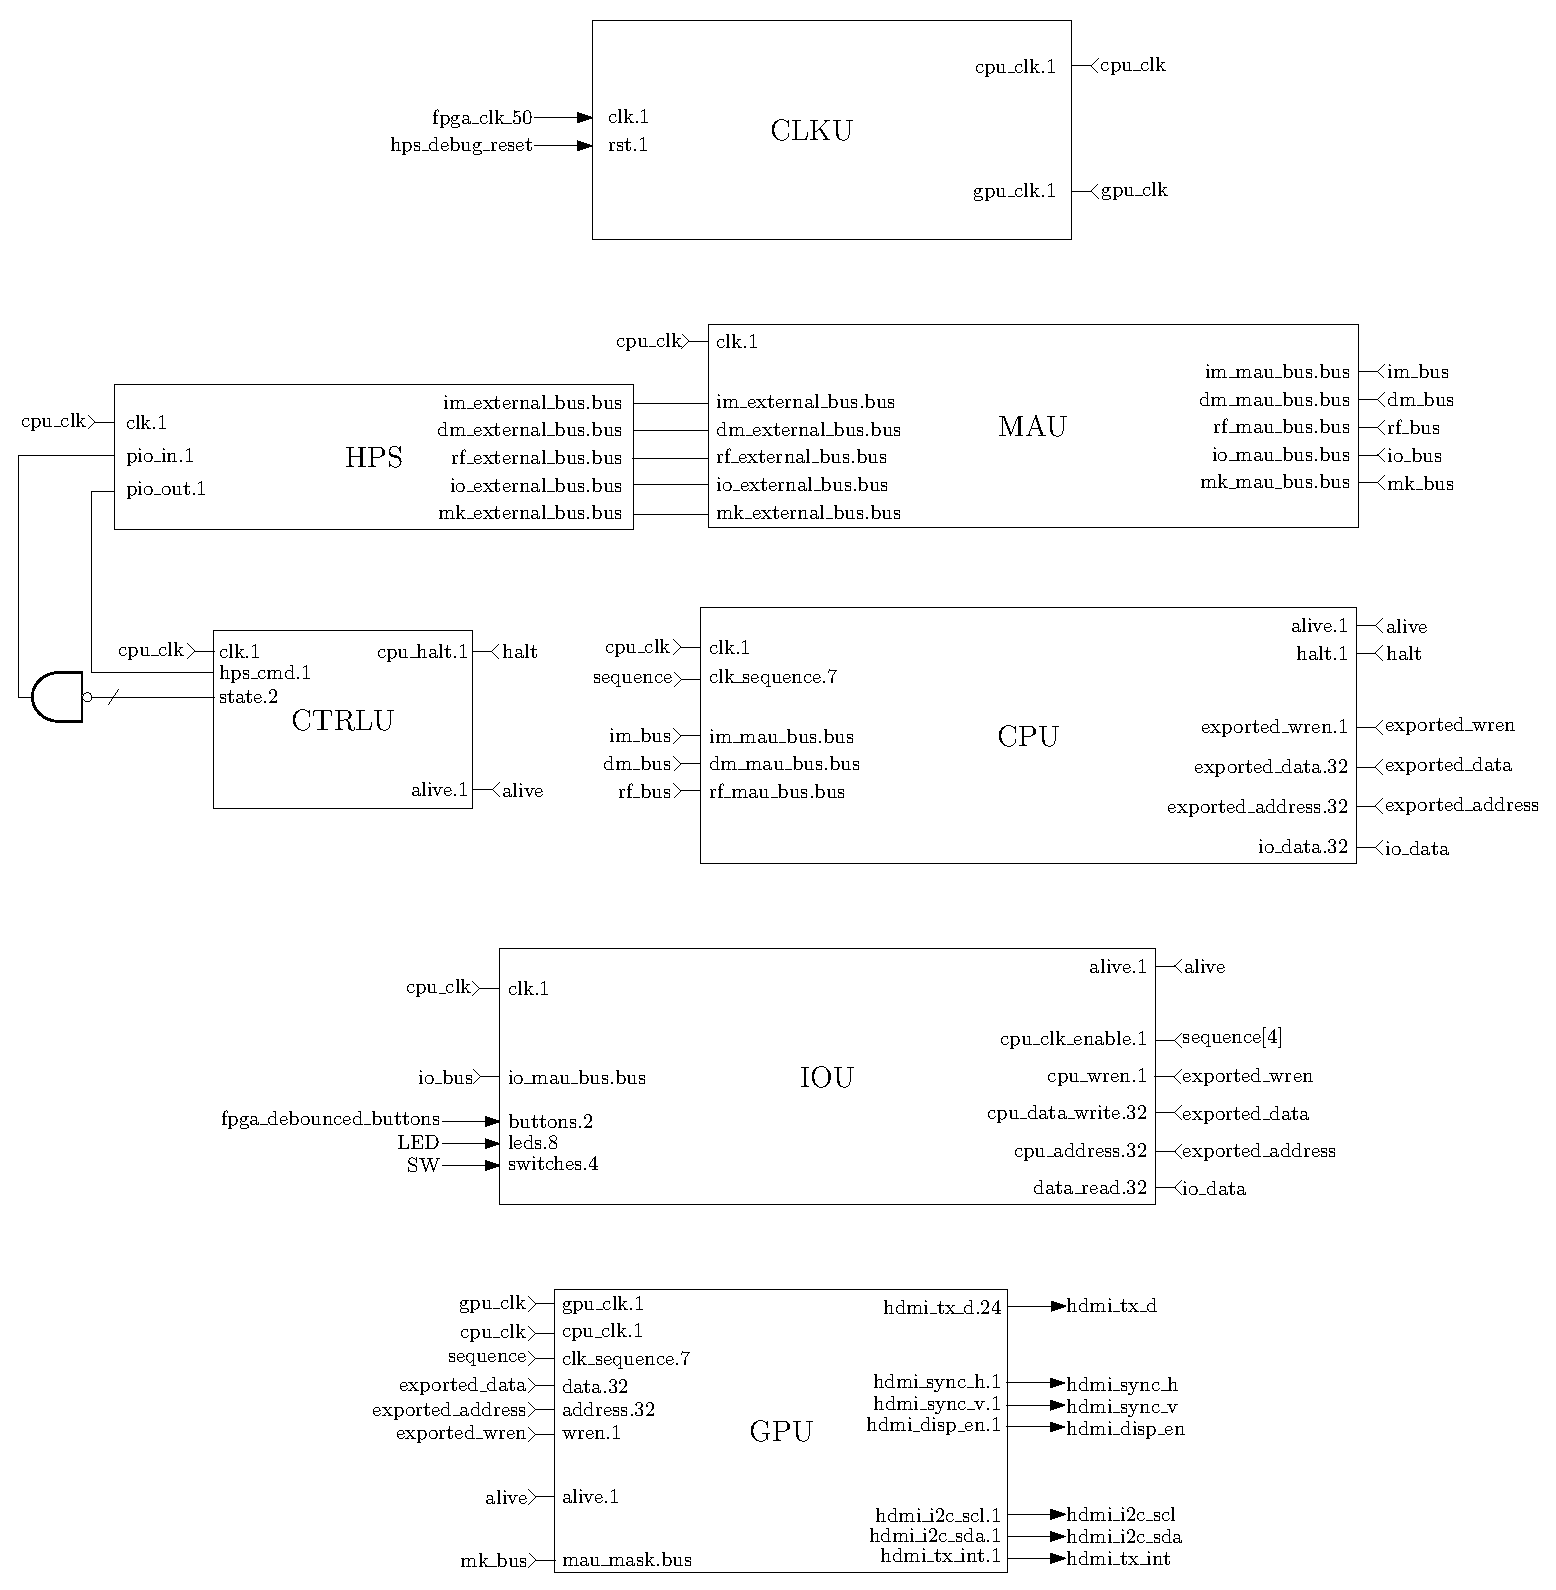
\includegraphics[width=\linewidth]{Chapter6-System/res/system.eps}
    \caption{Whole system.}
    \label{fig:system/system}
\end{figure}

\section{ARM side Operating System}

The ARM processor can be used in two ways. Either in bare metal where the programming is done 
directly in assembly on the processor. This method has the disadvantage of not being very 
accessible and of being expensive. The bare metal programming tools for the processor are not 
free and are professional licensed softwares. The second method is to install an operating system. 
This can be done by flashing an SD card that serves as storage for the ARM processor. On this card 
are created several partitions containing the bootloader (u-boot generally), the OS (Angström on 
the images of Terasic but any Linux can be adapted) and the programming file of the FPGA part. In 
this configuration, the bootloader configures the FPGA before launching the operating system. 

The image used to flash the SD card in this work is one provided by Intel using u-boot and ubuntu. The 
Terasic image containing Angström was also tested but this distribution is no longer maintained, so 
the image was not selected for use. The big disadvantage of the Intel image is that it takes up a 
lot more space, Ubuntu being much larger than an embedded Linux like Angström. It could be the work of 
another master thesis to improve the choice of the OS. Once the OS is installed and booted, one just 
has to program on it to be able to interact with the system on FPGA. This is the subject of the next 
section.
